\documentclass{osudissert96}
\usepackage{natbib}

% BibTeX from the BiBTeX Documentation
\def\BibTeX{{\rm B\kern-.05em{\sc i\kern-.025em b}\kern-.08em
    T\kern-.1667em\lower.7ex\hbox{E}\kern-.125emX}}

%
% It is better to break up the dissertation into multiple files (e.g.,
% one file per chapter, as well as separate files for the abstract,
% acknowledgements, and vita).  These files are brought into the
% document using \include{} statements.  There will be times, however,
% when you don't want to print the ENTIRE dissertation.  You can limit
% what will actually be printed by using the \includeonly{} statment.
% This contains a list of the files you want printed.  Any file NOT
% listed will not be printed.  However, all page numbers, references,
% etc., will be preserved as though all the files were actually
% printed. For example, the line below would result only in chapters 1
% and 3 being printed (if it were uncommented).
%

%\includeonly{ch_introduction}

% UPDATED TEXT (2010):
%  In the newest format, titles should be title case everywhere.
%
% HISTORICAL TEXT (1996):
%  In the new format, the titles of each chapter should appear in
%  uppercase.  In the TOC, however, they should be in lowercase.
%  The command below automates this behavior.  However, you'll have to be
%  careful not to include \labels within your \chapter definitions or
%  there will be problems.  If you don't want this to be automated, comment
%  out the \typesetChapterTitle definition below and do your chapters in
%  the form:
%  \chapter[MY TITLE]{My Title}
%
%  \renewcommand\typesetChapterTitle[1]{\uppercase{#1}}
\renewcommand\typesetChapterTitle[1]{#1}

\begin{document}

%
% First, declare the parts of your title page 
%

\author{Michael Crawley}
\title{Understanding the Aeroacoustic Radiation Sources and Mechanism in High-Speed Jets}
\authordegrees{B.S.}  % Degrees thus far, not including this one.
\unit{Department of Mechanical Engineering}

\advisorname{Mo Samimy}
\member{Datta Gaitonde}
\member{James Gregory}
\member{Mei Zhuang}      % Normally you will have advisor + 2 members


%
% The following creates the title page
%

\maketitle
\disscopyright


%
% Abstract goes here.
%

\begin{abstract}
  %  The dissertation abstract can only be 500 words.
It has been well-known within the aeroacoustic community that the dominant noise sources in high-speed turbulent jets are related to the large-scale structures which are generated in the initial shear layer by instabilities and which rapidly grow as they convect downstream.
However, the exact dynamics of these large-scale structures which are relevant to the noise generation process are less clear.
This work represents an attempt to study the dynamics and noise generated by the large-scale structures quantitatively and in high-fidelity in a Mach 0.9 turbulent jet using simultaneous pressure and velocity data acquisition systems alongside plasma-based excitation to produce coherent ring vortices in the shear layer.

In the first phase, the irrotational near-field pressure is decomposed into its constitutive acoustic and hydrodynamic components, and two-point cross-correlations are used between the acoustic near-field and far-field in order to identify the dominant noise source region.
Building upon the work of previous researchers, the decomposition is performed using a spatio-temporal wavelet transform, which was found to be more robust than previous algorithms.
Results indicated that for both individual as well as periodic large-scale structures, the dominant noise source region constitutes the upstream region of the jet, ending just before of the end of the potential core (in a time-averaged sense) in the unexcited jet.

The large-scale structure interactions were then investigated by stochastically-estimating the time-resolved velocity fields from the time-resolved near-field pressure.
For computational efficiency, the ensemble velocity snapshots were first decomposed into orthogonal modes, and the a mapping from the near-field pressure to the expansion coefficients was then produced using a feedforward neural network using backpropagation for learning.
The coherent structures generated by the excitation were then identified and tracked using standard vortex identification routines.
For the impulsively-excited jet, the individual structures quickly rolled up into a coherent structure within two jet diameters and then advected until roughly four jet diameters downstream, at which point it underwent a rapid disintegration.
For the periodically-excited jet, multiple smaller-scale structures are initially produced; these quickly merge into a single large-scale structure which matches the excitation wavelength.
Similar to the impulsively-excited structures, these now large-scale structures advect downstream and undergo a rapid disintegration near the end of the potential core. 

Finally, from Ribner's dilatation-based acoustic analogy the aeroacoustic source terms were computed using the time-resolved velocity field produced by the stochastic estimation.
Interpretation of the results is limited however, due to the number of assumptions and simplifications necessary for the computations, given the realities of the available experimental facilities.



\end{abstract}

\dedication{This work is dedicated to Science \ldots}


%
% Bring in Acknowledgement and Vita from separate files named ``ack.tex''
% and ``vita.tex''.
%

\begin{acknowledgements}
I should probably acknowledge someone here \ldots
\end{acknowledgements}


\begin{vita}

\dateitem{September 10, 1986}{Born - Plano, Texas}

\dateitem{2009}{B.S. Mechanical Engineering, \\
				University of Texas, Austin.}

\dateitem{2009-present}{Graduate Research Associate,\\
			 The Ohio State University.}


\begin{publist}

%% UPDATE FOR 2010:
%  Grad school only wants research publications, and it only wants those
%  research pubs that are actually published. Accepted or ``to appear''
%  publications don't count. If they look closely, they'll tell you to
%  remove any publications that aren't in print. Haivng said that, they
%  probably won't look that closely unless you put a really long list
%  here. You're tempting fate if you add instructional publications
%  though.

\researchpubs

\pubitem{\textbf{M. Crawley}, C.-W. Kuo, and M. Samimy,
\newblock ``Identification of the Acoustic Response in the Irrotational Near-field of an Excited Subsonic Jet.''
\newblock submitted to \emph{International Journal of Aeroacoustics}.}
	

\pubitem{\textbf{M. Crawley}, R. Speth, D. V. Gaitonde, and M. Samimy, 
\newblock ``A Study of the Noise Source Mechanisms in an Excited Mach 0.9 Jet - Complementary Experimental and Computational Analysis.''
\newblock AIAA Paper 2015-0736, \emph{53$^{rd}$ AIAA Aerospace Sciences Meeting}.}
	

\pubitem{\textbf{M. Crawley}, A. Sinha, and M. Samimy, 
\newblock ``Near-field and Acoustic Far-field Response of a High-Speed Jet Forced with Plasma Actuators.''
\newblock \emph{AIAA Journal}, expected 2015.}
	

\pubitem{\textbf{M. Crawley} and M. Samimy, 
\newblock ``Decomposition of the Near-Field Pressure in an Excited Subsonic Jet.''
\newblock AIAA Paper 2014-2342, \emph{20$^{th}$ AIAA/CEAS Aeroacoustics Conference}.}
	

\pubitem{\textbf{M. Crawley}, A. Sinha, and M. Samimy, 
\newblock ``Near-field Pressure and Far-field Acoustic Response of Forced High-Speed Jets.''
\newblock AIAA Paper 2014-0527, \emph{52$^{nd}$ AIAA Aerospace Sciences Meeting}.}	
	

\pubitem{\textbf{M. Crawley}, H. Alkandry, A. Sinha, and M. Samimy, 
\newblock ``Correlation of Irrotational Near-Field Pressure and Far-Field Acoustic in Forced High-Speed Jets.''
\newblock AIAA Paper 2013-2188, \emph{19$^{th}$ AIAA/CEAS Aeroacoustics Conference}.}
	

\pubitem{H. Alkandry, \textbf{M. Crawley}, A. Sinha, M. Kearney-Fischer, and M. Samimy,
\newblock ``An Investigation of the Irrotational Near Field of an Excited High-Speed Jet.''
\newblock AIAA Paper 2013-0325, \emph{51$^{st}$ AIAA Aerospace Sciences Meeting}.}
	

\pubitem{\textbf{M. Crawley}, M. Kearney-Fischer, and M. Samimy, 
\newblock ``Control of a Supersonic Rectangular Jet Using Plasma Actuators.''
\newblock AIAA Paper 2012-2211, \emph{18$^{th}$ AIAA/CEAS Aeroacoustics Conference}.}
\end{publist}



\begin{fieldsstudy}

	\begin{description}[style=multiline,leftmargin=1in,font=\normalfont]
		
		\item[Major Field:] Mechanical Engineering
		
		\item[Studies in:] High-speed Jets, Aeroacoustics, Flow Control, Fluid Mechanics, Optical Diagnostics, Wavelets, Reduced-Order Modeling
		
	\end{description}

\end{fieldsstudy}

\end{vita}




%
% Make the Table of Contents and other good stuff
%

\tableofcontents
\listoftables
\listoffigures


%
% The following is a list of chapters.  Each is brought in from a
% separate file using the \include{} command.
%

\chapter{Introduction}
\label{introduction}
\section{Motivation}
The advent of the turbojet engine led to a transformation in both commercial and military aviation, allowing for much faster flight than previously possible with propellor-driven aircraft. 
However, the increased thrust of turbojets has come at great cost; significant acoustic radiation is generated by the rotating components (compressor, turbine, fan), by the combustion process, and ultimately by the free jet itself. 
On the commercial side, the escalating number of flights, encroachment of urban and residential areas near airports, and tightening of environmental regulations have combined to force airports to institute curfews, surcharges and flight path restrictions to combat noise pollution. 
For the military, hearing damage inflicted on nearby personnel (particularly on aircraft carriers) has necessitated the implementation of noise reduction concepts on tactical aircraft.
During takeoff and landing, when acoustic radiation is most problematic to ground crew and  surrounding urban and residential areas, the dominant noise source of the jet engine is the aeroacoustic radiation generated by the high velocity engine exhaust.
This has spurred extensive research, spanning over six decades, into the acoustic source mechanism in high speed, high Reynolds number jets. 

While progress has been made in the field of aeroacoustics, both experimentally \citep{Tam1996, Viswanathan2006, Tam2008} as well as theoretically \citep{Cabana2008}, understanding of jet noise sources and their radiation mechanisms remains incomplete \citep{Jordan2008}.
This is due to the large number of interrelated parameters (e.g. Reynolds number, temperature ratio, acoustic Mach number, nozzle geometry, et cetera) as well as the large disparity in the associated length and time scales of the turbulent phenomena and the radiated noise.
Simulations of controlled free shear layers have suggested that there is significant potential for noise reduction, on the order of 11 dB in some cases [Wei 2006].
However, these simulations relied on non-physically defined actuation (that is, forcing was applied over a defined region by arbitrary energy, momentum, and body force terms), and a physical interpretation of the forcing parameters was not immediately clear to the researchers.
Current noise-mitigation technologies for free jets have largely been applied in an adhoc fashion, due to our incomplete understanding of the aeroacoustic sources.
Fully realizing this maximum noise reduction potential will require a much more detailed understanding of the mechanism (or mechanisms) by which free jets radiate to the far-field.

It is generally agreed that the dominant noise sources are related to the large-scale turbulent structures present in the mixing layer of the jet. 
What remains to be determined is what aspects of the large-scale structure evolution and interactions are relevant to the noise generation process. 
Theoretical models of spatially- and temporally-modulated wavepackets have shown great promise in replicating the observed characteristics of the dominant far-field noise [Cavalieri/Jordan?]. 
However, direct experimental data linking this structure evolution to the acoustic emission is still lacking. 
[FINISH?]
	
\section{Background}
\subsection{Flow Control}
TO DO:
	\begin{itemize}
		\item passive vs active flow control
		\item shear layer / jet instabilities
		\item large-scale structures / energy cascade / wavepackets
	\end{itemize}
\subsection{Components of Jet Noise}
A simplified model of the noise generation process in stationary free jets can be found in Fig. [INSERT FIGURE]. 
This model is based off of the work of Tam et al \citep{Tam1996, Tam2008}, who observed that the far-field spectra could be represented as a combination of two similarity spectra based on polar angle of the observer, regardless of jet Mach number or temperature.
At observer angles close to the jet downstream axis, the spectra exhibited a clearly defined spectral peak (\emph{F}-spectrum), whereas at sideline or upstream angles the spectra were broadband (\emph{G}-spectrum).
From this observation the two-component acoustic source model was born: fine-scale turbulence, dominant in the near-nozzle region, is responsible for the omni-directional acoustic radiation that dominates the sideline and upstream polar angles. On the other hand, the large-scale turbulent structures which exist further downstream produce the superdirective radiation that is readily apparent at aft polar angles. 
 
Additional noise source mechanisms have been identified for supersonic jets. In imperfectly expanded jets, shock cells are produced in the jet. As turbulent structures pass through these waves, the sharp pressure gradients cause them to emit acoustic radiation. 
This is observed directly in the far-field as a broad-band amplification at high frequencies, referred to simply as broad-band shock-associated noise (BBSAN). 
In stationary or subsonic airframes this radiation can generate a feedback loop, whereby the noise travels upstream to the nozzle exit, excites the initial shear layer, and produces new structures at the same frequency.
A high-amplitude, narrow-band tone (screech noise) is the end result of this feedback loop.
Lastly, supersonically-convecting (relative to the ambient) large-scale structures (which exist in supersonic and heated jets) produce high-amplitude, strongly-directional acoustic radiation towards aft angles.
This Mach wave radiation can be explained by a wavy-wall analogy (Tam again?).
In the present work, the jet is unheated and subsonic; as such these noise sources are not present and therefore neglected throughout the rest of this work.

TO DO:
	\begin{itemize}
		\item	Create simplified figure of free jet showing high frequency versus low frequency radiation (based off of Tam 2008)
		\item 	Explain Tam's "two-component" source model, with additional experimental evidence?
	\end{itemize}

\subsection{Acoustic Source Models}
By rearranging the Navier-Stokes equations, Lighthill \citep{Lighthill1952} was able to transform the governing equations for fluid dynamics into an inhomogeneous convected wave equation. 
In this acoustic analogy, the source term comprises Reynolds stress, shear stress, and density fluctuation terms (commonly referred to as \emph{Lighthill's stress tensor}).
As this formulation is exact (aside from the assumption of a constant sound speed), complete knowledge of the source field will yield an exact solution for the acoustic far field.
In practical applications (e.g. high-speed, turbulent jets) however, the full source field cannot be measured using current experimental capabilities nor simulated with sufficient fidelity, thereby requiring certain simplifications.
       
\chapter{Experimental Methodology}
\label{methodology}

\section{Anechoic Chamber}

\section{Data Acquisition}

\section{LAFPAs as Diagnostic Tools}
\chapter{Near-field Signature of Aeroacoustic Sources}
\section{Preprocessing: Filtering the Actuator Self-Noise}  
\chapter{Estimation of Time-resolved Velocity Fields}
\label{sect:velocity}
Analysis of the evolution, interaction, and disintegration of the large-scale structures, and ultimately the noise generated thereby, is greatly simplified by the acquisition of time-resolved flow-field measurements.
Furthermore, as will be explained in \sect{sect:source}, computation of the aeroacoustic source field from a simplified acoustic analogy will require time-resolved flow-field data.
Unfortunately, directly acquiring time-resolved velocity fields for the jet currently under study is simply not possible due to the combination of a large domain of interest ($0 \leq z/D \lesssim 12, 0 \leq r/D \lesssim 3$) and high characteristic frequencies on the order of several kHz.
Full-field, high-fidelity measurement techniques capable of this repetition rate simply do not exist at present.
An indirect method is therefore required in order to estimate the evolution of the large-scale structures, in a reduced-order sense.

Phase-locking of a data acquisition system to a reference signal (such as an actuator or a naturally occurring resonance tone) is a common experimental technique; by varying the delay between the trigger and time of data acquisition, multiple phases can be acquired and the coherent component of the phenomena can be analyzed.
Phase-locking of the PIV system to the LAFPAs was initially considered for the present work, but quickly discarded.
Sample analysis performed using a numerical database indicated that a very high temporal resolution was required in order to accurately compute fluctuation rates in the dilatation field (the relevance of which will become more apparent in the following chapter).
At moderate to high excitation frequencies, this was feasible, though potentially tedious (for example, $\sim$16 phases were estimated as necessary at $St_{DF} =0.25$).
At $St_{DF} =0.05$ however, this would require roughly \textit{forty} phases (the significant dead time between actuations means that it is not necessary to acquire the entire range of phases from $0$ to $2\pi$, but this is small consolation).
Clearly, a more efficient data acquisition method is in order.
\section{Stochastic Estimation}
Stochastic estimation was first proposed by Adrian \citep{Adrian1977} in 1977, as an outgrowth from the conditional statistical analyses popular at the time. 
Large-scale coherent structures had been educed from anisotropic turbulent flows (such as boundary or shear layers) by conditional sampling techniques.
Adrian succeeded in identifying detailed flow structures (`conditional eddies') in isotropic turbulence by computing a mean-square estimate of the flow from linear two-point correlations (higher-order, nonlinear correlations were explored in Adrian \citep{Adrian1979}). 
The methodology was extended in Adrian \citep{Adrian1994} to estimation of velocity fields using spatial correlations coupled with a reduced set of measurements.

Stochastic estimation attracted considerable attention from the fluid dynamics community due to its potential to educe meaningful structures and behavior from highly turbulent, incoherent flows as well as its relative simplicity.
Subsequent researchers refined stochastic estimation in several important aspects.
Bonnet \etal \citep{Bonnet1994} developed the complementary technique by combining linear stochastic estimation (LSE) with proper orthogonal decomposition (POD), improving the accuracy due to higher correlation levels between low-order modes.
The estimated velocity fields produced by LSE were projected onto the POD eigenfunctions (computed from the random, non-time-resolved velocity fields) to produce an estimate of the time-dependent POD coefficients, which can then be used to reconstruct low-order representations of the estimated random velocity field.
Picard \& Delville \citep{Picard2000} used LSE and POD to link the longitudinal pressure distribution surrounding a low subsonic jet to vortical motions in the shear layer by simultaneously sampling microphone and hotwire data.
In Boree \citep{Boree2003} the POD coefficients of the velocity field were estimated directly, using pressure modes.
Ewing \& Citriniti \citep{Ewing1997} extended the standard form of LSE, in which spatial correlations are computed at a single time lag, by Fourier transforming the reference signal in time prior to computing the two-point cross-correlations (now cross-spectra). 
The incorporation of phase-delay information over a range of frequencies (and in essence, including information from multiple time lags) was found to significantly improve the accuracy of the reconstructions for many flow regimes \citep{Ewing1997,Tinney2006,Tinney2008b}.
Finally, multi-time-delay LSE-POD was performed in the physical domain (as opposed to the Fourier) by Durgesh \& Naugton \citep{Durgesh2010} to study the turbulent structures in a near wake region.

The current work borrows heavily from the methodology of Tinney \etal \citep{Tinney2008b} and Sinha \etal \citep{Sinha2010} in order to estimate the two-component time-resolved velocity field on a streamwise slice of the jet.
As explained in \sect{sect:piv_method}, two-component PIV snapshots were acquired at well-defined instants of experimentally recorded near-field pressure traces.
The computational methodology by which the stochastic estimation is performed has been modified, however.
Complementary stochastic estimation is used, due to its significantly lower computational cost as well as theorized improvement in accuracy.
Thus, the instantaneous velocity fields will be separated into characteristic modes via POD and the time-dependent modal coefficients, rather than the velocity fields themselves, will be estimated using SE.
Instead of performing the stochastic estimation using either linear or higher-order cross-correlations (or cross-spectra), the conditional mapping between the near-field pressure and the POD modal coefficients will be generated by an artificial neural network with multi-time-delay.
Artificial neural networks were chosen over the more traditional cross-correlations due to their simplicity compared to high-order methods as well as their demonstrated ability to model nonlinear processes in turbulent flows \citep{Lasagna2015}.

\subsection{Stochastic Estimation via Artificial Neural Networks}
Artificial neural networks (ANNs), are statistical computing models which developed as a branch of machine learning.
The design of neural networks is based on simplified models of the human brain: they are comprised of a large number of simple, interconnected computing cells (`neurons') and therefore are massively parallel distributed processors.
The neurons themselves are based on models of biological neurons, and produce a single output based on the linear summations of inputs (either directly from the user or from other, lower-level neurons) and synaptic weights which is then modulated by a nonlinear activation function.
The synaptic weights are modified by a learning algorithm in order to minimize a cost function; this generally takes the form of explicit training (supervised learning).
The interconnectivity of a massive number of these nonlinear computing cells allows artificial neural networks to approximate unknown, nonlinear functions of an arbitrary number of inputs while retaining a certain, elegant, simplicity.
It should be unsurprising then, that ANNs have already been applied for the estimation and control of a variety of turbulent flow regimes.
Interested readers are recommended to refer to Haykin \citep{Haykin1994} for an extensive background on artificial neural networks, their developmental history, and many additional network structures not used in this work.

A feedforward network structure was used in the current work, a schematic of which can be found in \fig{fig:ch4_neural_net}.
The ANN was comprised of an input layer, to which near-field pressure traces were supplied, a single hidden layer, and an output layer which produced estimates of the time-varying POD coefficients. 
The hidden and output layers were fully connected, and the modified logistic function (hyperbolic tangent) was used as the activation function.
The pressure traces were centered around the acquisition of a PIV image group, and was downsampled to 100 kHz in order to match the frequency response of the microphones.
The record time supplied for each training block was $\pm 5.12$ microsecond; this was determined by estimating the time delay for a large-scale structure to convect through the experimental domain (the convective velocity of the large-scale structures was conservatively estimated as $U_c \simeq 0.5 U_j$).
\begin{figure}
	\centering
	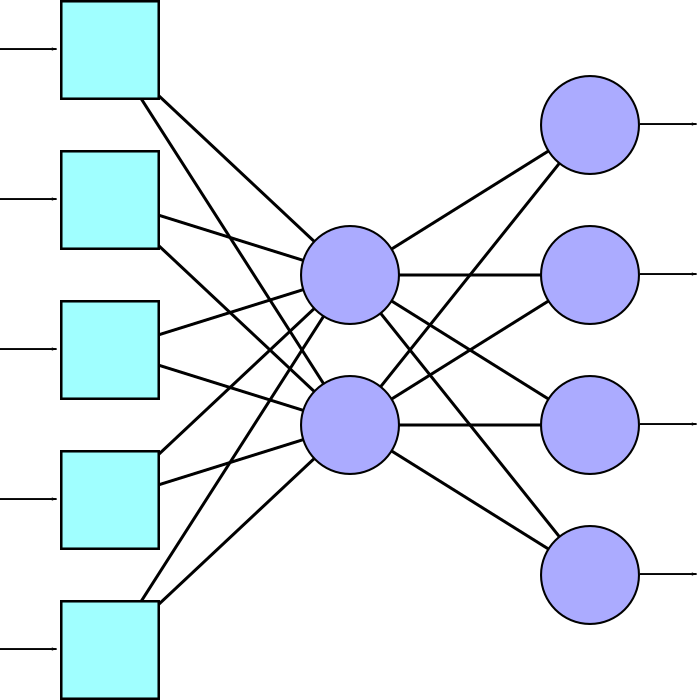
\includegraphics[width = 2.5in]{Figures/neural_net_v2.png}
	\caption{Schematic of a feedforward ANN with a single hidden layer. The activation function is applied only to the hidden and output layers. The number of neurons depicted in each layer is meant to represent the \textit{relative} number used by the actual ANN.}
	\label{fig:ch4_neural_net}
\end{figure} 

POD modes and time-varying coefficients were computed from the velocity fields using the method of snapshots \citep{Sirovich1987}; the kernel was defined as the two-component turbulent kinetic energy.
The instantaneous velocity fields were not preprocessed prior to the decomposition (that is, missing or spurious vectors were not replaced or interpolated).
As experimental noise in the velocity fields will be completely uncorrelated to the near-field measurements, it will be filtered out by the stochastic estimation and hence preprocessing is unnecessary.
Unlike many past researchers, the coefficients for every POD mode were estimated, rather than just the most energetic modes, for two reasons.
First, it is not guaranteed that an individual POD mode corresponds to a physically distinct turbulent flow structure or event - an event may be broken up into multiple POD modes of varying energy levels.
Secondly, the most energetic POD mode(s) is not necessarily the most relevant mode(s) for the acoustic generation process (see Jordan \etal \citep{Jordan2007} for a modification to the standard POD kernel in order to mitigate this issue). 

Even though the network is estimating even the least-energetic modes, the current method is far more computationally efficient than directly estimating the velocity fields themselves.
By encoding spatial correlations in the POD expansion coefficients, estimation of the $N$ snapshots of $M \times K$ spatial locations has been reduced from a minimization problem of $N$ vectors of $2MK$ to one of $N$ vectors of $N$.
For the current experimental database, this means the system has been reduced from $290,508 \times 1500$ to $1500 \times 1500$.
The neural network now only needs to identify the temporal correlations between the pressure field and the individual POD coefficients; it does not need to learn the spatial correlations.

Learning was accomplished via the standard backpropagation method \citep{Haykin1994}, which approximates the error surface of the cost function using first-order derivatives; the error `propagates' backwards from the output neurons to the hidden neurons and the synaptic weights at each neuron are updated to identify the (hopefully, global) minimum of the cost function using gradient descent.
The cost function was defined as the mean-squared-error between the predicted and measured expansion coefficients for a given PIV image group.
The velocity field, $\mathbf{U}$ at a given instance, $k$, can be recovered from $N$ orthonormal modes, $\phi$, and time-varying expansion coefficients, $a_k$, as $\mathbf{U} = \sum_{n=0}^{N} a_{k}^{n} \phi^n$ \citep{Berkooz1993}.
The total energy of each mode is therefore encoded in $a_k^n$, which will serve as a simple energy weighting for the cost function (the importance of relative errors to the cost function will essentially be scaled by the energy in each particular mode).
Training of the network was performed using the roughly 1500 ensemble pressure-velocity blocks of data (a few PIV images in each set had to be discarded due to laser misfires); synaptic weights were updated based on the average of all blocks (batch processing) using a constant learning rate.
A well-known issue with the gradient descent optimization method is that it has a tendency to get trapped in local minima and fails to converge to the global minimum.
Therefore, sample results were also calculated using a much different learning algorithm: adaptive particle swarm optimization.
Details will not be presented here however, as the results were found to not differ substantially from those produced by the backpropagation algorithm (while requiring significantly higher computational resources).

\subsection{Reduced-Order Representation of the Flow-Field}
Ultimately, due to limitations both in the methodology as well as in the ability of the microphones located outside the flow to sense fine-scale turbulent fluctuations, the estimated velocity field is going to represent a reduced-order model of the jet.
This can be easily observed in \fig{fig:ch4_SEPOD_filtering}, where the measured axial velocity field at an arbitrary instance in time has been plotted against the velocity field produced by the SE-POD estimation from the near-field pressure at the same instance in time.
For comparison purposes, a reduced-order reconstruction of the measured velocity field from the first 100 POD modes (but without estimating from the near-field pressure using SE) has also been included.
Note that here the output of the model produced by SE-POD is being compared against a known output that the system is meant to match; this is not an evaluation of the \textit{predictive} power of the model but of the \textit{representative} power.
\begin{figure}
	\centering
	\begin{subfigure}{0.75\textwidth}
		\centering
		\includegraphics[width=0.95\linewidth]{Figures/ch4_Ux_true.png}
		\caption{Measured}
	\end{subfigure}\\
	\begin{subfigure}{0.75\textwidth}
		\centering
		\includegraphics[width=0.95\linewidth]{Figures/ch4_Ux_estimated.png}
		\caption{Estimated}
	\end{subfigure}
	\begin{subfigure}{0.75\textwidth}
		\centering
		\includegraphics[width=0.95\linewidth]{Figures/ch4_Ux_POD100.png}
		\caption{First 100 POD modes}
	\end{subfigure}
	\caption{Comparison of a raw instantaneous axial velocity field $St_{DF} =0.05$ (a) against the same velocity field estimated from the near-field pressure (b) and finally a reduced-order reconstruction of the raw velocity using the first 100 POD modes ; units are in m/s.}
	\label{fig:ch4_SEPOD_filtering}
\end{figure}

As one would hope, the large-scale turbulent fluctuations are correctly identified by the SE-POD algorithm, and a mapping from the near-field pressure to this structures is appropriately generated.
The accuracy in the feature reproduction degrades considerably however as the scale of the turbulent eddy is reduced.
Some small-scale behavior is retained though most is filtered out, particularly the downstream region.
This was entirely expected however, as the reference signal is much more strongly damped with wavenumber than the conditional field being estimated (decay rates of $-20/3$ for the pressure field versus $-5/3$ in log-space for the velocity field).
The pressure field simply does not have the resolution to approximate the velocity field, particularly further downstream where the microphones are further from the jet centerline due to the spreading of the shear layer.
The estimated velocity fields are specifically referred to in the present work as \textit{reduced}-order rather than \textit{low}-order however.
Comparison of the estimated velocity against a reconstruction of the measured field using the most energetic 100 POD modes (of a total of 1500 POD modes corresponding to the 1500 uncorrelated velocity fields) indicates that the SE-POD algorithm retains similar (if not greater) energy levels.
An example of this is the small-scale structure observed at $z/D \simeq 8$, just outside the high-velocity region of the jet (orange, in the figure in the measured velocity.
This distinct structure is still visible (though smeared and slightly reduced in amplitude) in the estimated velocity, though it is basically nonexistent in the 100-mode reconstruction which contains $\sim 50$\% of the fluctuating energy (see \fig{fig:ch4_modal_energy}).
While it is unlikely that this particular structure is notably important to the acoustic emission of the jet, low modal energy modulations of the large-scale structures may be.
Hence, it is desirable to retain as much of the information as possible when estimating the flow.

As a side note, the measured velocity fields retain some experimental errors from the PIV data processing; for instance, the small pockets of zero axial velocity observed on lower shear layer (particularly for $2 < z/D < 4$) in \fig{fig:ch4_SEPOD_filtering} are non-physical and correspond to missing vectors. 
As these experimental errors will be completely uncorrelated from the pressure signals, a conditional reconstruction will have great difficulty in reproducing them; in fact they \textit{should not} map from the pressure to the velocity at all.

It is also important to be mindful that an individual POD mode may not in fact correspond to anything physically distinct in the turbulent flow - it is after all, merely a mathematical construct which is based on no \textit{a priori} information of the system under investigation.
Tinney \etal \citep{Tinney2008b} found that the modes produced by (spectral) POD had a tendency to appear in coupled pairs, and similar behavior is observed herein. 
For reference, the ten most energetic POD modes are shown in \fig{fig:ch4_St005_PODmodes} for $St_{DF} = 0.05$ and \fig{fig:ch4_St025_PODmodes} for $St_{DF} = 0.25$.
The characteristic scales of the excitation induced structures are smaller than the actual excitation period, as a result a significant amount of dead time occurs between LAFPA pulses during which the flow returns to its unperturbed state.
Because of this, analysis methods based on ensemble-averages of the velocity field show little difference between the baseline and $St_{DF} = 0.05$ excited jets (for this reason, the POD modes for the baseline jet are not shown).

For the impulsively-excited ($St_{DF} = 0.05$) jet, the dominant orthogonal modes are concentrated downstream of the end of the potential core, and it is not until mode 8 that a clear symmetric pattern about the jet centerline emerges. 
(However, it should be noted that modes 4 and 5 are very nearly mirrors of each other, and as such could produce symmetric features if coupled.)
Clearly, the excited axisymmetric structures represent only a small portion of the turbulent kinetic energy of the jet, and as such low-order representations of the flow will fail to accurately capture their dynamics.
As the excitation frequency is increased, the LAFPA-induced structures become high-energy periodic oscillations in the jet shear layer and core, and the POD modes are modified accordingly (\fig{fig:ch4_St025_PODmodes}).

Strong, axisymmetric fluctuations are now observed in the jet core for the first two POD modes, which match the wavelength of the excited structures (assuming $U_c \simeq 0.7 U_j$, per the two-point near-field correlations of Crawley \etal \citep{Crawley2015}) and which peak in amplitude near the end of the potential core.
The structure of mode 2 is quite similar to that of mode 1, differing only by a phase shift of $\pi/2$. 
This is a numerical artifact produced by the downstream convection of the large-scale structures (remember that while multiple time-delays have been incorporated into the stochastic estimation algorithm, the POD was computed using a single time-delay out of necessity).
Interestingly, some of the higher modes, particularly mode 10, exhibit core fluctuations at a harmonic of the excitation wavelength.
As will be seen shortly, LAFPA excitation at this frequency yields higher-frequency structures which undergo a periodic merging to ultimately generate structures at the excitation frequency. 
These modes are capturing this process which might be highly relevant to the noise generation process. 
Lastly, even in the periodically-excited jet where the LAFPA-induced structures are the dominant POD modes, the modal energy convergence (\fig{fig:ch4_modal_energy}) of the POD modes is rather slow; as mentioned previously, 100 of the 1500 modes are required in order to capture 50\% of the total energy.
The relatively slow convergence of the modal energies, not only in the impulsively-excited jet but particularly in the periodically-excited jet, was something of a surprise for the researcher.
The convergence rate is of course a function of the number of snapshots used in the decomposition, however these results indicate that even in the excited jet, the highly coherent large-scale structures are a small fraction of the overall turbulent kinetic energy.
Again, this speaks to the necessity of accurately estimating not just the low-order modes, but the high-order as well.
\begin{figure}
	\centering
	\includegraphics[width=1\linewidth]{Figures/ch4_St005_POD_Modes.png}
	\caption{First 10 POD modes (axial component only) for $St_{DF} = 0.05$, ordered top-down and then left-right.}
	\label{fig:ch4_St005_PODmodes}
\end{figure}
\begin{figure}
	\centering
	\includegraphics[width=1\linewidth]{Figures/ch4_St025_POD_Modes.png}
	\caption{First 10 POD modes (axial component only) for $St_{DF} = 0.25$, ordered top-down and then left-right.}
	\label{fig:ch4_St025_PODmodes}
\end{figure}
\begin{figure}
	\centering
	\includegraphics[width=3in]{Figures/ch4_POD_energies.png}
	\caption{POD modal energy convergence.}
	\label{fig:ch4_modal_energy}
\end{figure}


\section{Large-Scale Structure Interactions}
\subsection{Global Flow-Field Effects}
The global effects of excitation on shear layer development, both in general and in particular for LAFPAs, has been well-documented in the literature already (see Samimy \etal \citep{Samimy2012} for a review on LAFPA excitation in jets).
Therefore, only the features relevant to the current work will be briefly covered here.
Excitation produces highly-energetic structures which entrain the ambient fluid surrounding the shear layer, thus increasing mixing between the high-momentum core fluid and the ambient fluid.
As a result, the growth rate of the shear layer can be amplified significantly; this is illustrated in \fig{fig:ch4_shearlayerspreading}.
Excitation near the jet column mode ($St \simeq 0.35$) produces a rapid spreading of the initial shear layer until $z/D \simeq 5$, after which the spreading rate returns to the natural spreading rate.
(A quick note about the axial velocity fields shown in \fig{fig:ch4_shearlayerspreading}: the twelve circular regions of low velocity aligned on the outer edge of the lower shear layer are experimental artifacts. Laser reflections off of the microphones saturated the cameras, thus precluding the possibility of computing cross-correlations for these locations. Contrary to how it might appear in this figure, the microphone array is not in the flow-field, but situated behind from the cameras' point of view.)
\begin{figure}
	\centering
	\begin{subfigure}{0.75\textwidth}
		\centering
		\includegraphics[width=0.95\linewidth]{Figures/ch4_St000_Um.png}
		\caption{Baseline}
	\end{subfigure}\\
	\begin{subfigure}{0.75\textwidth}
		\centering
		\includegraphics[width=0.95\linewidth]{Figures/ch4_St035_Um.png}
		\caption{$St_{DF} = 0.35$}
	\end{subfigure}
	\caption{Effect of excitation on the shear layer spreading rate, as visualized by the axial component of the velocity field.}
	\label{fig:ch4_shearlayerspreading}
\end{figure}

The increased mixing also affects the high-velocity side of the shear layer, resulting in a reduction in the length of the potential core.
In \fig{fig:ch4_centerlinemach}, the time-averaged centerline Mach number for each excitation case (as well as the natural jet) has been plotted as a function of axial distance.
A slow progression in the location of the end of the potential core is clearly evident, with it shifting upstream from $z/D \simeq 6$ eventually to $z/D \simeq 5$ as the excitation Strouhal number nears the jet preferred frequency of $St_{DF} \simeq 0.35$ (though not shown here, above this excitation frequency the effect is reduced).
The end of the potential core is of particular interest for the current work, as previous researchers have indicated that the dominant noise generation mechanism is associated with the violent breakdown of large-scale axisymmetric structures as they pass through this location \citep{Hileman2005}.
The two-point correlations of \sect{sect:nearfield}, which identified the dominant noise source region as occurring near the end of the potential core, hint at this as well.

The breakdown of the large-scale axisymmetric structures occurs because as the shear layers merge, the interface between the interior sides of the ring vortex becomes highly unstable, so any small perturbations quickly grow and destroy the vortex.
The exact location at which this breakdown occurs is ultimately going to be a function of structure growth rate, as larger structures will self-interact further upstream.
The location of the end of the potential core is therefore dependent on the passage of the large-scale structures, and hence is not strictly constant in time [who to cite here?].
Therefore, an axial shift in the time-averaged acoustic source (or a source location not exactly at the time-averaged end of potential core) is not necessarily reflective of a changing source mechanism, but may instead simply indicate that the source mechanism is now occurring at a different location.
\begin{figure}
	\centering
	\includegraphics[width = 3.5in]{Figures/ch4_centerlineMach.png}
	\caption{Centerline Mach number for all excitation cases; baseline jet is indicated by `0.00'.}
	\label{fig:ch4_centerlinemach}
\end{figure}

\subsection{Large-Scale Structure Disintegration}
Hileman \etal \citep{Hileman2005} investigated the evolution and interactions of large-scale structures and ultimately how these relate to the noise generation process in a supersonic, ideally-expanded jet by combining time-resolved flow visualizations with a three-dimensional microphone array.
Their results showed that the dominant noise was being generated near the end of the potential core, in the region where the shear layers merged.
Large-amplitude, highly-intermittent acoustic events were found to be associated with a fluctuation in the length of the potential core, which the authors ultimately speculated was related to the passage and finally the rapid disintegration of large-scale coherent structures just downstream of the end of the potential core.
The results of \sect{sect:nearfield} also indicated that the jet core region was responsible for the dominant acoustic generation in a subsonic jet, at least to low angles with respect to the jet axis.
The dynamics of the large-scale structures in this region, namely the structure disintegration, are therefore of particular concern to the current work.

Vortex identification was performed by computing the swirling strength at each instance in the estimated velocity field; details and justification for this method can be found in Adrian \etal \citep{Adrian2000}.
The evolution of the impulsively excited ($St_{DF} = 0.05$) vortex ring has be tracked in \fig{fig:ch4_impulse_structure_disintegration}.
For ease of visualization, a two-dimensional, five-point boxcar filter was applied to the estimated velocity fields prior to computing the swirling strength, and the results have been phase-averaged based on the recorded LAFPA trigger signal over roughly 30 excitation periods.
Lastly, a solid red line has been overlain to approximately match the convective velocity of the structures.
Only a select number of phases are shown here, as a significant amount of dead time between excitations occurs due to the mismatch in the spatial and temporal characteristic frequencies of the large-scale structures.
\begin{figure}
	\centering
	\includegraphics[width=5in]{Figures/ch4_St005_lambda.png}
	\caption{Evolution of the independent vortex ring ($St_{DF}=0.05$), as visualized using swirling strength. Images are shown at constant phase steps of roughly $\pi/8$, starting with a phase of $\pi/4$.}
	\label{fig:ch4_impulse_structure_disintegration}
\end{figure}

As already known from prior experiments at the GDTL \citep{Kearney-Fischer2009}, the excitation produces a strong roll-up of vortical (toroidal) fluid in the near-nozzle region; in the present case the large-scale structure generated by the excitation is clearly discernible over the background turbulence (and experimental/computational noise) by $z/D \simeq 1$.
If the contours of the swirling strength field are to be believed, the rapid growth of the vortex slows by $z/D \simeq 1.5$ and it advects downstream relatively unchanged until  $z/D \simeq 4$ (other vortex identification methods, such as Q-criterion or $\lambda_2$-criterion, were also investigated and a general agreement was found, though swirling strength produced the visually-simplest fields).
It is at this point that the vortex undergoes a rapid disintegration, yielding smaller scale, less coherent structures (though by no means would these structures be classified as fine-scale turbulence) as it passes through the end of the potential core.
These results are in general agreement with those of Hileman \etal \citep{Hileman2005}, who found that the large-amplitude acoustic bursts of energy were associated with the passage of high-order structures through the end of the potential core.
\begin{figure}
	\centering
	\begin{subfigure}{1\textwidth}
		\centering
		\includegraphics[width=3.5in]{Figures/ch4_centerline_mach_temporal.png}
		\caption{}
		\label{fig:ch4_centerlinemach_temporal}
	\end{subfigure}\\
	\begin{subfigure}{1\textwidth}
		\centering
		\includegraphics[width=3.5in]{Figures/ch4_rawUx_acceleration.png}
		\caption{}
		\label{fig:ch4_St005_rawUx_snapshot}
	\end{subfigure}
	\caption{Fluctuations associated with the passage of large-scale structures in the axial velocity along the jet centerline at $z/D = 4$ (a) and an arbitrary raw PIV snapshot displaying similar behavior for the $St_{DF}  = 0.05$ jet(b).}
\end{figure}

Accompanying the passage of the vortical structure is a large amplitude oscillation in the axial velocity, which reaches into the potential core to the jet centerline (which is expected, given the radial profile of axisymmetric instability waves known from linear stability analysis \citep{Michalke1965}).
As shown in \fig{fig:ch4_centerlinemach_temporal}, the vortical structures are characterized by large velocity deficit, which is preceded by a large acceleration of the fluid that often crosses the sonic threshold as the vortex begins to disintegrate.
The author was surprised to see such a strong axial acceleration, however this same axial acceleration can also be found in the raw PIV snapshots that have not been post-processed by SE-POD if one looks for it (note the coherent region of supersonic velocity just upstream of $z/D = 4$ in \fig{fig:ch4_St005_rawUx_snapshot}).
An acceleration of the less-coherent structures can also be observed in \fig{fig:ch4_impulse_structure_disintegration}, as the small eddies are located further downstream in the final frames than they would be if following a constant convective velocity (as denoted by the red line overlain on the frames).
As discussed by Tam \citep{Tam1996} (among others), the aeroacoustic efficiency of structures increases with Mach number and envelope modulation.
Therefore, the twin effects of rapid disintegration (\ie rapid envelope modulation) and acceleration around $z/D \simeq 4$ would to greatly enhance the acoustic efficiency from the vortex.
This potentially explains why the region in which the turbulent structure rapidly disintegrates appears to dominate over the region in which the turbulent structure rapidly grows in terms of the noise emission per the results of \sect{sect:nearfield}.

\subsection{Coherent Structure Merging}
In the simulated subsonic shear layer of Wei \& Freund \citep{Wei2006}, optimized control for noise mitigation using generalized actuation was implemented using the adjoint perturbation method.
The methodology was able to affect a significant reduction in the emitted noise, though the exact mechanism by which this was accomplished was not immediately clear, even in this highly simplified flow (two-dimensional shear layer).
In Cavalieri \etal \cite{Cavalieri2010b} the same numerical database was investigated with a specific focus on identifying intermittent events related to the noise generation process.
Here it was found that the control achieved the majority of the sound reduction by suppressing a single triple vortex interaction, thereby regularizing the flow and preventing the generation of high-amplitude peaks in the acoustic field.
The results of Bridges \& Hussain \citep{Bridges1992} and Kibens \citep{Kibens1980} also identified vortex pairing as a prominent noise source in a (low) subsonic jet.
With this in mind, the evolution of the vortices in the periodically excited jets was analyzed.

\fig{fig:ch4_period_structure_disintegration} illustrates a complete excitation period for the $St_{DF} = 0.25$ excited jet; as before the velocity fields were smoothed prior to computation of the swirling strength, and the results have been phase-averaged.
Previous analysis of the near-field had used two-point correlations between subsequent microphones in order to estimate the convective velocity of the large-scale structures; based on the time-lag for the maximum correlation value, the convective velocity was estimated as $U_c \simeq 0.7 U_j$.
However, the analysis of Speth \citep{Speth2015} in a simulated Mach 0.9 unheated jet found that this method over-predicted the convective velocity; for example, near the end of the potential core two-point correlations in the irrotational near-field produced an estimate of $U_c \simeq 0.67 U_j$ whereas correlations in the \textit{flow}-field produced an estimate of $U_c \simeq 0.64 U_j$.
Essentially, the energy of the acoustic field in the irrotational near-field though small, is non-trivial, and as a result the much higher propagation velocity for the acoustic energy skews the convective velocity estimate to slightly higher values.
By using only the hydrodynamic component of the near-field (produced by the decomposition of \sect{sect:ac_decomp}), the convective velocity was estimated as $U_c \simeq 0.54 U_j$ near the nozzle exit and $U_c \simeq 0.65 U_j$ near the end of the potential core (which, incidentally, are nearly identical to the values reported in Speth \citep{Speth2015}).
Based on these values, the vortex spacing is expected to range from $\lambda \simeq 2.3D$ at the nozzle exit to $\simeq 2.6D$ near the end of the potential core.
\begin{figure}
	\centering
	\includegraphics[width=5in]{Figures/ch4_St025_lambda.png}
	\caption{Evolution of the periodic vortex ring ($St_{DF}=0.25$), as visualized using swirling strength. One complete actuation period is shown.}
	\label{fig:ch4_period_structure_disintegration}
\end{figure}

As expected, the excitation produces a periodic roll-up of large-scale structures which, in the downstream region of the potential core, roughly match with the vortex spacing for this frequency (see frame 1 in \fig{fig:ch4_period_structure_disintegration}).
However, in the upstream region ($z/D < 2$) the vortex spacing halves - the LAFPA excitation is in fact producing multiple structures per actuation pulse.
In frame 2, the harmonic structures at $z/D = 1$ are beginning to pair.
The trailing structure is inducted inside the preceding structure, and by $z/D \simeq 3$ the pairing process is complete; the appearance of structures now matches the excitation frequency.
The physical interpretation of POD mode 10 in \fig{fig:ch4_St025_PODmodes} is now obvious: the orthogonal decomposition is identifying the harmonic structures and their coherent merging in the upstream region of the jet.
As the resultant structure convects downstream, the beginning of the breakdown of the vortex is witnessed near $z/D \simeq 4$, similar to the results of the impulsively excited vortex ring and an acceleration of the centerline velocity to slightly supersonic speeds is also observed (\fig{fig:ch4_centerlinemach_temporal}).
Here however, a secondary interaction between structures appears to be occurring, most visibly in frames 5--7. 
As the vortex at $z/D \simeq 4.5$ is breaking down, the trailing vortex does as well, in fact much more abruptly than the leading vortex.
As the cycle is repeated (beginning again at frame 1), these two vortices (or more accurately, the less coherent, higher-order remnants of them) are no longer individually distinguishable.

Clearly (and unsurprisingly), the vortex interactions in the periodically excited jet are far more complex than the impulsively excited jet.
However, as was seen both in terms of the far-field response (\fig{fig:ch3_farfield}) as well as the acoustic source region estimated from the decomposed near-field (\fig{fig:ch3_xcorrOA}), the acoustic fields for $St_{DF}=0.05$ and $St_{DF}=0.25$ show remarkable similarity, at least at angles close to the jet axis.
Therefore, this implies that the added complexity of the periodic excitation (harmonic structures, vortex pairing) are not the primary drivers for noise emission (though they may still play a lesser role).
Rather, the consistent, rapid breakdown of the LAFPA-induced structures near $z/D \simeq 4$ and accompanying fluid acceleration in both excited jets appears to be the dominant noise source. 
In order to more conclusively link this behavior to the noise emission directly, in \sect{sect:source} the aeroacoustic source term will be calculated from the estimated time-resolved velocity fields using a simplified form of Lighthill's acoustic analogy.
\chapter{Dilatation as the Aeroacoustic Acoustic Source}
Ribner presented an alternative approach to Lighthill's acoustic analogy which posited fluctuating fluid dilatations as the source of aeroacoustic emission.
\section{Numerical Method}
\subsubsection{Helmholtz Decomposition}
	For a given vector field, $\vec{F}$, Helmholtz's theorem states that any sufficiently smooth vector field can be linearly decomposed into irrotational and solenoidal vector fields, as
	\begin{equation}
	\vec{F} = \vec{F}_{potential} + \vec{F}_{rotational} = \nabla \Phi + \nabla \times \Psi
	\end{equation}
	where $\Phi$ is a scalar field and $\Psi$ is a vector field.
	From basic vector calculus properties, we can therefore compute these solenoidal and irrotational components by taking the divergence of this equation, leading to:
	\begin{equation}
	\nabla \cdot \vec{F} = \nabla^{2} \Phi
	\end{equation}
	which is simply Poisson's equation, where in the context of velocity decomposition the forcing term is simply the divergence of the flow field.
	Since we are unable to acquire gradients in the azimuthal coordinate, we are going to drop this term, leaving
	\begin{equation}
	\frac{\partial U_r}{\partial r} + \frac{\partial U_z}{\partial z} + \frac{U_r}{r} = \frac{1}{r} \frac{\partial \Phi}{\partial r} + \frac{\partial^2 \Phi}{\partial r^2} + \frac{\partial^2 \Phi}{\partial z^2} 
	\end{equation}
	
	The solution procedure is therefore to first compute $\Phi$, then add the gradient of this field to the raw velocity vector field in order to produce the solenoidal velocity field.
\subsubsection{Pseudo-Pressure Solver}
\subsubsection{Wavelet Denoising}
\section{Wavepackets in the Pseudo-Pressure Field}
\chapter{Conclusions}
The aeroacoustic mechanisms in high-speed, turbulent jets were investigated using simultaneous pressure and velocity measurements of large-scale structures generated by plasma excitation.
As the focus of this work was on mixing noise generated by turbulent shear layer structures common to all flow regimes, rather than acoustic emission generated by supersonic flow phenomena, an unheated, Mach 0.9 jet was used.
In the current work, only structures of azimuthal mode zero (axisymmetric ring vortices) were investigated. Previous researchers have identified the axisymmetric mode as the dominant acoustic emission pattern, and this also served to simplify the data acquisition and analysis greatly by eliminating the need to obtain azimuthal velocity components and gradients.

To begin with, the irrotational near-field pressure was linearly decomposed into it's constitutive hydrodynamic and acoustic components, akin to the work of previous researchers \citep{Tinney2008}.
Here though, the pressure was filtered via a two-dimensional, spatio-temporal wavelet transform, which was found to be more robust than the Fourier transform used previously.
Once decomposed, linear correlations between the far-field acoustic signal at $30^\circ$ and the acoustic component of the near-field were computed in order to identify the dominant acoustic source region in the jet based on the measured time-lag for the peak correlation.
In all cases, natural and excited jets, the dominant acoustic source region was found to comprise the upstream region of the jet and end at $z/D \simeq 4$, just upstream of the end of the potential core.
This result is in general accordance with previous results acquired at the GDTL by Hileman \etal \citep{Hileman2005}, which identified the acoustic source region using delay-and-sum beamforming with a circular microphone array in the acoustic near-field (that is, far enough such that hydrodynamic pressure effects are negligible, but not in the true geometric far-field of the jet).
In that work, the dominant acoustic source region for an unheated, Mach 1.3 jet was found to be located just downstream of the end of the potential core, and was related to the breakup of large-scale coherent structures as they passed through this region.

The evolution, interactions, and, disintegration of the large-scale structures induced by the plasma excitation were then studied by stochastically-estimating the time-resolved velocity fields from temporally-correlated velocity snapshots and near-field pressure traces.
The velocity snapshots were first decomposed into orthogonal modes and expansion coefficients per Sirovich's method of snapshots for proper orthogonal decomposition \citep{Sirovich1987}.
A mapping from the near-field pressure to the POD expansion coefficients was generated by a standard feedforward, backpropagating neural network; from this mapping the time-resolved expansion coefficients could be estimated and thus a reduced-order, time-resolved estimate of the velocity field produced.
At very low excitation frequencies (impulsive excitation) each plasma pulse generates a single dominant structure, which initially grows rapidly as it convects downstream. 
As the structure nears the end of the potential core, $z/D \simeq 4$, a rapid disintegration of the vortex is observed, coincident with a strong axial acceleration.
As the excitation frequency is increased, a much more complex structure evolution takes form.
At moderate excitation frequencies (periodic forcing), multiple structures are initially formed by the plasma pulse; these quickly merge to form periodic structures which match the excitation frequency.
These structures later undergo a rapid disintegration and acceleration, similar to the impulsive excitation structures, as the convect downstream near the end of the potential core. 

Finally, the aeroacoustic sources were estimated from the time-resolved velocity fields using Ribner's simplified form of Lighthill's acoustic analogy, which relates fluctuations in the dilatation field to fluctuations in the acoustic field.
This required numerous simplifications to the governing equations, which ultimately degraded the accuracy of the computed aeroacoustic source field.
Unfortunately, this limited interpretation of the results, as the computed far-field acoustic signal did not match well with the measured signal.
It had been hoped that high-resolution velocity fields and nonlinear estimation methods would be sufficient for overcoming the challenges inherent in measuring acoustic source fields in high-speed, turbulent jets, but clearly this was not the case. 
An experimentalist can always dream, though.

% % %What do the final results show????

% %Future work section
Perhaps the greatest deficiency in the current work was the reliance on linear correlations from the acoustic component of the near-field to the far-field.
This was done because two-point correlations are quick, simple, and their use is well-established in the literature.
However, this overlooks the great advancements in acoustic holography that have occurred in the last several decades.
Though the linear array of microphones used in this work is not well-optimized for acoustic beamforming, additional information on the noise source characteristics, such as directivity or frequency content, can likely be gleaned from the decomposed irrotational near-field using a number of beamforming algorithms of varying complexity.
Readers interested in acoustic beamforming are referred to the work of Papamoschou \citep{Papamoschou2011}.

%\appendix
%\include{app1}


%
% The all important bibliography file at the end of your document!! Use
% the bibstyle you (your department) like in the \bibliographystyle{}
% statement and list the name of your bibliography database file in
% the \bibliography{} statement.  In this example, ``bibfile.bib'' is
% the name of the database.  See the LaTeX manual appendix B for details
% about the bibliography database and BibTeX.
%

\bibliographystyle{plain}
\bibliography{new_master}

\end{document}




